\chapter{Analisis}
\label{chap:analisi}

Pada bab ini dibahas mengenai analisis aplikasi sejenis, analisis kebutuhan aplikasi, analisi kontrol yang dipakai, analisis terhadap siklus hidup aplikasi, analisis peta, analisis pemanfaatan sumber data, analisis Kiri API, diagram \textit{Use Case}, dan diagram kelas.

%Analisis Aplikasi Sejenis
\section{Analisis Aplikasi Sejenis}
\label{lab:Analisis Aplikasi Sejenis}
% Aplikasi publik transport Android
\hspace{0.5cm} Aplikasi sejenis yang ditemui bernama Public Transport\footnotemark[1]. Namun aplikasi Public Transport tersebut hanya dapat dijalankan pada sistem aplikasi android. Aplikasi Public Transport ini memanfaatkan Kiri API yang penggunaannya sederhana. Di halaman awal pengguna dapat mengetik lokasi asal dan tujuan. Selain dengan mengetik pengguna juga dapat menunjuk lokasi pada peta. Setelah lokasi dipilih sistem memastikan dengan memberi daftar nama jalan dan tempat terkait. Jika sudah memilih maka sistem mengeluarkan hasil pencarian rute.
\footnotetext[1]{\url{https://play.google.com/store/apps/details?id=travel.kiri.smarttransportapp}}

Berikut adalah tampilan dari aplikasi Public Transport (Gambar ~\ref{fig:home} sampai ~\ref{fig:peta}):

\begin{figure}[h]
	\centering
		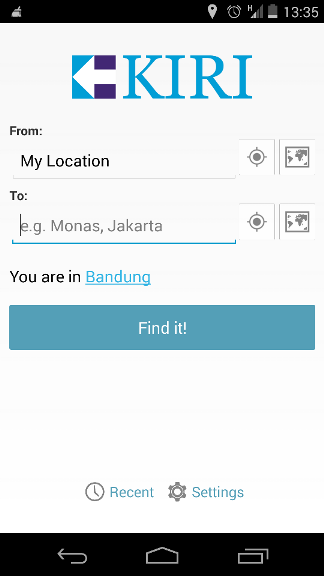
\includegraphics[scale=0.5]{Gambar/KIRI_Android/home}
	\caption{Tampilan Utama Aplikasi Public Transport}
	\label{fig:home}
\end{figure}

Gambar ~\ref{fig:home} menunjukan halaman utama aplikasi Public Transport. Di halaman ini pengguna dapat memasukan lokasi asal dan lokasi tujuan. Cara memasukan lokasi ada 2 macam yaitu dengan mengetik dan menunjuk pada peta dengan mengetuk tombol peta. Bila pengguna ingin menunjuk lokasi pengguna berada dapat dilakukan dengan menunjuk lokasi pada peta lalu menekan tombol untuk memilih koordinat. Tersedia juga pilihan kota yang dapat dipilih oleh pengguna.

\begin{figure}[h]
	\centering
		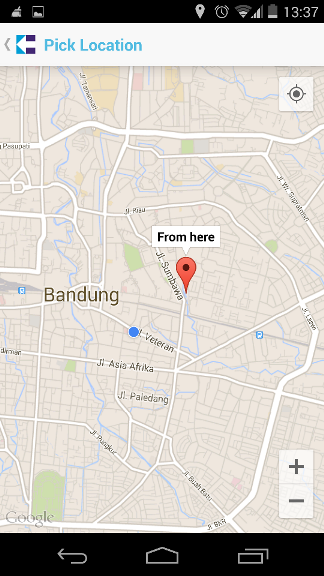
\includegraphics[scale=0.5]{Gambar/KIRI_Android/menunjuk_lokasi}
	\caption{Menunjuk Lokasi pada Peta}
	\label{fig:menunjuk}
\end{figure}

Gambar ~\ref{fig:menunjuk} jika pengguna sudah mengetahui lokasi namun tidak tahu nama lokasi. Pada halaman ini pengguna diarahkan untuk menemukan lokasi pada peta memilihnya.

\begin{figure}[h]
	\centering
		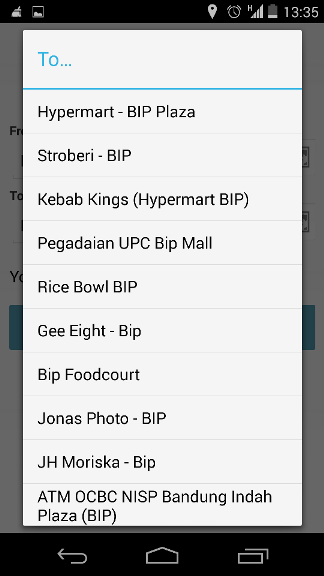
\includegraphics[scale=0.5]{Gambar/KIRI_Android/terkait}
	\caption{Memberikan Daftar Nama Tempat dan Nama Jalan Terkait}
	\label{fig:terkait}
\end{figure}

Pada gambar ~\ref{fig:terkait} pengguna dapat memilih nama tempat terkait. Pemilihan didasarkan sesuai masukan pengguna untuk memastikan tempat asal maupun tempat tujuan. Jika nama tempat sudah jelas maka tidak ada halaman yang menampilkan nama tempat.

\begin{figure}[h]
	\centering
		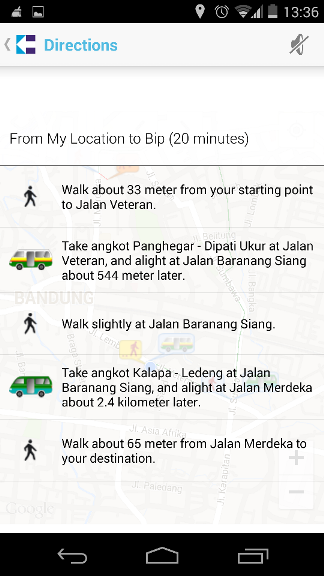
\includegraphics[scale=0.5]{Gambar/KIRI_Android/tampilan_daftar}
	\caption{Tampilan Rute Kendaraan Umum dalam Bentuk Daftar}
	\label{fig:daftar}
\end{figure}

Pada gambar ~\ref{fig:daftar} menampilkan daftar rute kendaraan umum yang harus dinaiki beserta gambar untuk mempermudah pengguna. Selain itu disertakan juga jarak dan perkiraan waktu sampai di lokasi tujuan.

\begin{figure}[h]
	\centering
		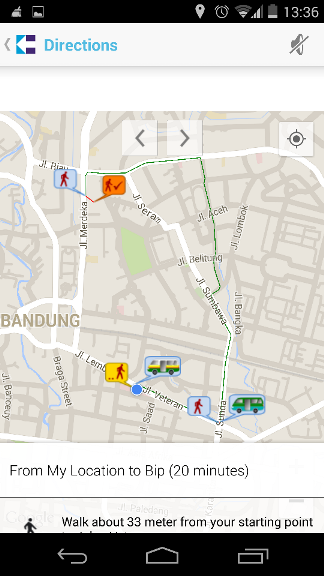
\includegraphics[scale=0.5]{Gambar/KIRI_Android/tampilan_peta}
	\caption{Tampilan Rute Kendaraan Umum di Peta}
	\label{fig:peta}
\end{figure}
\newpage
Pada gambar ~\ref{fig:peta} menampilkan rute kendaraan umum dan jalur yang harus dilalui pada peta. Dengan cara ini pengguna dapat mengetahui posisi dan jalur yang harus dilalui.

% tampilannya, cara kerja, hal yang dapat dilakukan

%Analisis Analisis Program
\section{Analisis Aplikasi}
\label{lab:Analisis Aplikasi}
\hspace{0.5cm} Aplikasi dibuat menggunakan bahasa pemograman C\#. Aplikasi yang digunakan untuk membangun Aplikasi Pencari Rute Kendaraan Umum untuk Windows Phone adalah Visual Studio Express 2012. Pada sub-bab ini dibahas kebutuhan aplikasi, anaslisis kontrol yang dipakai, analisis terhadap siklus hidup aplikasi, analisis peta, analisis pemanfaatan sumber data, analisa Kiri API, diagram \textit{use case}, dan diagram kelas dari aplikasi yang dibangun. 

%Analisis Kebutuhan Aplikasi
\subsection{Kebutuhan Aplikasi}
\label{lab:Kebutuhan Aplikasi}
\hspace{0.5cm} Dari hasil observasi dalam menentukan lokasi asal dan lokasi tujuan ada dua cara. Kedua cara tersebut yaitu dengan menulis alamat atau tempat dan dengan menunjuk pada peta. Cara menuliskan alamat atau tempat yaitu dengan menuliskan alamat atau tempat pada tempat yang disediakan untuk asal dan tujuan. Cara menunjuk pada peta yaitu dengan menunjuk peta pada koordinat yang diinginkan. Kedua hal tersebut pada dasarnya sama saja tetapi ada faktor kemudahan pengguna dalam pemakaiannya. Jadi aplikasi menyediakan dua cara tersebut dengan tujuan agar pengguna dapat memilih salah satunya.

Pada saat menuliskan lokasi atau tempat atau menunjuk langsung pada peta mungkin saja terjadi kesalahan. Kesalahan tersebut bisa saja disebabkan salah pengetikan atau nama tempat yang tidak ada. Maka dari itu dibutuhkan pemeriksaan terhadap masukan pengguna. Pemeriksaan tersebut dilakukan setelah pengguna memulai pencarian dengan menekan tombol "FIND".

Untuk hasil keluaran ada dua tipe seperti aplikasi peta lainnya. Kedua tipe tersebut adalah bentuk daftar dan bentuk peta. Bentuk daftar memudahkan dalam melihat tiap langkah rute. bentuk peta memudahkan pengguna dalam melihat arah dan posisi lingkungan pada rute yang dipilih.

\hspace{0.5cm} Berdasarkan kebutuhan aplikasi diatas maka aplikasi yang dibangun didasarkan pada kebutuhan sebagai berikut.
\begin{enumerate}
	\item Pengguna dapat memasukan lokasi asal dan lokasi tujuan pada \textit{textbox} yang disediakan atau menunjuk langsung lokasi pada peta.
	\item Mendapatkan lokasi terkait menurut lokasi yang dimasukan pengguna.
	\item Menampilkan hasil rute angkutan umum dari lokasi asal ke lokasi tujuan.
\end{enumerate}

% SUB Analisis Kontrol yang Dipakai
\subsection{Analisis Kontrol yang Dipakai}
\label{lab:Analisis Kontrol yang Dipakai}
\hspace{0.5cm} Dari kebutuhan yang telah disebutkan diatas disadari pentingnya kontrol yang harus dipakai. Kontrol yang dimaksud termasuk tata letak, teks, pilihan, dan daftar. Kebutuhan kontrol penting bukan hanya untuk kebutuhan tapi memudahkan pengguna.

Untuk kontrol tata letak dibutuhkan pengaturan yang tertata rapih dan beberapa elemen dalam satu baris atau kolom. Penggunaan kontrol tata letak yang rumit tidak diharapkan dalam aplikasi karena akan membingungkan pengguna. Dari hasil pengamatan kontrol tata letak yang cocok adalah tata letak \textit{grid}. Kontrol tata letak ini dipilih karena mudah diposisiskan sesuai baris dan kolom. Kelebihan tata letak \textit{grid} adalah menyesuaikan jika layar diputar dari posisi pemandangan ke posisi potret dan sebaliknya.

Kontrol terhadap teks juga diperlukan untuk aplikasi. Kebutuhan yang diperlukan adalah mengeluarkan potongan teks yang dapat dibaca dan tempat pengguna memasukan teks. Untuk mengeluarkan teks yang dapat dilihat pengguna diperlukan penggunakan \textit{textblock}. \textit{textblock} digunakan untuk menampilkan tulisan "from" dan "to" pada halaman utama aplikasi. Untuk masukan pengguna, aplikasi menyediakan \textit{textbox} sebagai tempat masukan teks. \textit{textbox} digunakan sebagai masukan untuk lokasi asal dan lokasi tujuan.

Suatu aplikasi tentunya tidak hanya mempunyai satu halaman, aplikasi yang dibuat memiliki beberapa halaman yang mempunyai tugas berbeda. Karena hal tersebut dibutuhkan kontrol untuk berpindah dari satu halaman ke halaman lain. Kontrol yang dibutuhkan yaitu kontrol tombol. Kontrol tombol mengeksekusi \textit{event click} yang memungkinkan pindah halaman dan melakukan perintah. Kontrol tombol digunakan untuk berpindah ke halaman peta, menemukan lokasi pengguna, dan pencarian rute. Pada halaman utama terdapat 5 buah dengan penjelasan sebagai berikut.
\begin{itemize}
	\item Tombol "map" pada bagian from\\
	Tombol untuk berpindah dari halaman utama menuju halaman peta. Pada halaman peta pengguna dapat menunjuk lokasi asal dan kembali lagi ke halaman utama. Saat kembali ke halaman utama lokasi yang dipilih akan disimpan dan pada \textit{TextBox} bagian from akan tertulis "Maps".
	\item Tombol "here" pada bagian from\\
	Tombol untuk mancari lokasi pengguna. Setelah tombol ini di tekan maka lokasi pengguna akan disimpan dan pada bagian \textit{TextBox} bagian from akan tertulis "Here".
	\item Tombol "map" pada bagian to\\
	Tombol untuk berpindah dari halaman utama menuju halaman peta. Pada halaman peta pengguna dapat menunjuk lokasi tujuan dan kembali lagi ke halaman utama. Saat kembali ke halaman utama lokasi yang dipilih akan disimpan dan pada \textit{TextBox} bagian to akan tertulis "Maps".
	\item Tombol "here" pada bagian to\\
	Tombol untuk mancari lokasi pengguna. Setelah tombol ini di tekan maka lokasi pengguna akan disimpan dan pada bagian \textit{TextBox} bagian to akan tertulis "Here".
	\item Tombol find\\
	Tombol ini akam mencari rute angkutan umum dan menampilkannya pada halaman peta.
\end{itemize}

Pada aplikasi ini ditampilkan daftar tempat dan daftar rute angkutan umum yang dipakai. Bentuk daftar digunakan karena hasil tempat dan rute angkutan umum yang ditampilkan cukup banyak jumlahnya. Bentuk daftar yang dapat dipakai di Windows Phone adalah menggunakan \textit{ListBox}. \textit{ListBox} menampilkan daftar tempat dan daftar rute satu per satu menurun ke bawah.

% SUB Analisis Terhadap Siklus Hidup Aplikasi
\subsection{Analisis Terhadap Siklus Hidup Aplikasi}
\label{lab:Analisis Terhadap Siklus Hidup Aplikasi}
\hspace{0.5cm} Aplikasi pada Windows Phone memiliki siklus hidup yang dijelaskan pada bab ~\ref{subsec:Siklus Hidup Aplikasi}. Pengaturan aplikasi ini diatur sesuai konfigurasi awal sistem operasi Windows Phone. Tetapi pengaturan ini dapat diatur sesuai kebutuhan aplikasi. Karena di aplikasi ini terdapat keadaan yang berbeda dengan konfigurasi awal sistem operasi Windows Phone maka perlu dilakukan pengaturan ulang siklus hidup.

Saat aplikasi dijalankan, pengguna memasukkan lokasi asal dan lokasi tujuan. Setelah memasukkan lokasi pengguna lalu mencari rute. Ketika rute berhasil ditemukan maka aplikasi berada di keadaan Running. Tetapi ada kemungkinan pengguna berpindah aplikasi atau mematikan layar untuk menghemat daya. Dalam kasus tersebut sistem operasi Windows Phone menganggap aplikasi tidak aktif dan aplikasi masuk pada keadaan \textit{dormant}. Untuk menangani kasus tersebut maka aplikasi harus menyimpan keadaan dan informasi sesaat sebelum aplikasi menjadi tidak aktif. Penanganan yang digunakan adalah menyimpan keadaan sebelumnya di memori.

Pada saat aplikasi masuk keadaan Dormant semua \textit{thread} dan proses akan dihentikan. Pada saat tersebut juga GPS Windows Phone terhenti dan tidak akan mengetahui posisi pengguna. GPS akan kembali aktif mengetahui posisi pengguna jika pengguna masuk ke aplikasi dan tentunya membutuhkan waktu untuk pelacakan lokasi. Tetapi Windows Phone mendukung proses di belakang untuk pelacakan GPS selama keluar dari aplikasi atau layar perangkat dimatikan. Maka dari itu aplikasi yang dibuat harus mendukung pengaksesan lokasi meskipun layar perangkat dimatikan atau berpindah aplikasi. 

Ketika aplikasi sudah berada pada keadaan \textit{Dormant} atau \textit{Tombstoned}, pengguna masih dapat memulihkan keadaan aplikasi saat aplikasi berada di keadaan \textit{Running} sebelumnya. Penanganan yang dilakukan untuk hal tersebut adalah menggunakan \textit{method} OnNavigatedTo(). Menggunakan \textit{method} tersebut bertujuan memulihkan informasi halaman pada keadaan \textit{Running} sebelumnya.
%mendukung backgorund execution, running bacground event

% SUB Analisis Peta
\subsection{Analisis Peta}
\label{lab:Analisis Peta}
\hspace{0.5cm} Untuk tampilan peta ada beberapa aspek yang perlu diperhatikan untuk memudahkan pengguna. Aspek yang perlu diperhatikan adalah sebagai berikut.
\begin{itemize}
	\item Pemetaan terhadap peta atau \textit{cartographic} dan mode warna
	\item Tingkat \textit{zoom}
	\item Menampilkan gambar dan keterangan angkutan umum menggunakan \textit{pushpin}
	\item Menggambar rute pada peta menggunakan \textit{polyline}
\end{itemize}

Untuk cara pandang peta terdapat 4 pandangan yang disediakan peta di Windows Phone yaitu \textit{Road}, \textit{Aerial}, \textit{Hybrid}, dan \textit{Terrain}. Aplikasi ini adalah aplikasi pencari rute dan pandangan lebih banyak diarahkan ke jalanan perkotaan. Kebutuhan pengguna adalah nama jalan, kondisi jalan, dan kondisi sekitar. Dari dasar pandangan tersebut pandangan yang dipilih untuk aplikasi ini adalah \textit{Road}. Tambahan setelah mengatur pandangan peta yaitu mengatur warna dan menggunakan mode warna terang sesuai bawaan peta di Windows Phone.

Tampilan awal peta di Windows Phone akan mengeluarkan peta dengan pandangan dunia. Karena aplikasi pencarian rute ini masih terbatas di Pulau Jawa, Indonesia terutama Jawa Barat maka tingkat \textit{zoom} harus diatur agar mengikuti lokasi pengguna dan di satu daerah saja. Jika pengguna berada di daerah Bandung maka tingkat \textit{zoom} pada peta disesuaikan pada daerah tersebut. Tingkat \textit{zoom} dapat dapat diatur dari kode dan XAML. Tingkat \textit{zoom} yang digunakan adalah 14. Tingkat \textit{zoom} 14 menampilkan satu kota dengan jelas.
%kasih gambar zoom 14

Di setiap kota ada satu angkutan umum yang banyak dipakai yaitu angkutan kota(angkot). Namun bagi yang baru pertama mengunjungi suatu daerah dan mencari angkot mungkin akan mengalami kesulitan membaca trayek/rute dari angkot tersebut. Namun ada satu cara yang mudah untuk membedakan angkot di setiap rute yaitu dari warna dan coraknya. Agar dapat memudahkan pengguna dan menghindari pengguna dari kesalahan naik angkot maka Kiri API sudah menyediakan gambar angkot yang seusai dengan setiap rute. Gambar angkot tersebut akan ditempatkan di peta dengan suatu penampung beserta keterangannya. Salah satu teknik untuk menempatkan gambar tersebut adalah dengan membuat lapisan terpisah di atas peta tempat gambar tersebut. Untuk hal tersebut dimanfaatkan \textit{pushpin} sebagai lapisan terpisah untuk menaruh gambar dan keterangan angkutan umum. Berikut tampilan \textit{pushpin} untuk angkot~\ref{fig:pushpin_angkot} dan \textit{pushpin} untuk jalan kaki~\ref{fig:pushpin_jalan}.

\begin{figure}[h]
	\centering
		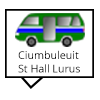
\includegraphics[scale=0.5]{Gambar/out_kiri/angkot}
	\caption{Tampilan \textit{Pushpin} untuk Angkot}
	\label{fig:pushpin_angkot}
\end{figure}

\begin{figure}[h]
	\centering
		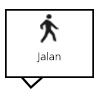
\includegraphics[scale=0.5]{Gambar/out_kiri/jalan}
	\caption{Tampilan \textit{Pushpin} untuk Jalan Kaki}
	\label{fig:pushpin_jalan}
\end{figure}

Pencarian rute yang digunakan untuk aplikasi yaitu dengan memakai Kiri API. Kiri API memberikan kembalian berupa titik-titik rute perjalanan dari lokasi asal ke lokasi tujuan. Karena hal itu aplikasi harus menggambar rute tersebut sesuai jalan pada peta. Untuk hal tersebut digunakan \textit{polyline} pada Windows Phone untuk menggambarnya. \textit{Polyline} yang digambar harus terlihat dengan jelas dan diberi warna yang kontras dengan tampilan peta. Warna polyline yang dipilih adalah merah dengan ketebalan 4.

% SUB Analisis Pemanfaatan Sumber Data
\subsection{Analisis Pemanfaatan Sumber Data}
\label{lab:Analisis Pemanfaatan Sumber Data}
\hspace{0.5cm} Aplikasi yang dibuat memanfaatkan sumber data dari luar. Sumber data yang didapatkan dalam format JSON (\textit{Javascript object Notation}). Pengambilan sumber data tersebut dilakukan dengan melakukan permintaan melalui protokol HTTP dengan parameter \textit{Uniform Resource Identifier} / URI. 

Untuk dapat memanfaatkan sumber data di Windows Phone perlu memanfaatkan kelas HttpClient.\textit{Method} yang digunakan adalah GetStringAsync(). \textit{Method} ini mengirimkan permintaan dengan parameter URI dan hasil yang dikembalikan memiliki tipe data \textit{string}. Karena \textit{method} ini mengembalikan hasil dalam tipe data \textit{string} maka mudah disesuaikan dengan kebutuhan tugas akhir ini. Selanjutnya agar data dalam bentuk \textit{string} tersebut dapat dimanfaatkan maka diperlukan proses \textit{Deserialization}. Proses \textit{Deserialization} dimaksudkan untuk mengubah bentuk \textit{string} ke objek. Untuk melakukan \textit{Deserialization} perlu memanfaatkan \textit{library} Json.NET. Aplikasi memanfaatkan \textit{library} Json.NET karena memiliki performa yang baik. Untuk hal tersebut aplikasi yang dibuat perlu menggunakan \textit{method} DeserializeObject().
%penggunaan getString

% SUB Analisis Kiri API
\subsection{Analisis Kiri API}
\label{lab:Analisis Kiri API}
%parameter get karena hanya untuk mendapatkan data dan tidak ada data sensiti yg dikirimkan.
\hspace{0.5cm} Kiri API menyediakan 2 jenis permintaan yaitu \textit{POST} dan \textit{GET}. Dalam tugas akhir ini digunakan protokol \textit{GET} untuk melakukan permintaan. Permintaan \textbf{GET} dipilih karena dalam tugas akhir ini aplikasi banyak mendapatkan data dan tidak ada data sensitif yang dikirimkan. Untuk hal ini maka mengirim ke URI \url{http://kiri.travel/handle.php}.

Untuk setiap permintaan terhadap Kiri API dibutuhkan \textit{API key}. Kegunaan \textit{API key} adalah password untuk mengakses Kiri API. \textit{API key} dapat didapatkan di \url{dev.kiri.travel}. \textit{API key} yang digunakan pada tugas akhir ini adalah 97A7A1157A05E***. %97A7A1157A05ED6F
     
Untuk tugas akhir ini digunakan 2 layanan yang ada pada Kiri API. Layanan yang digunakan adalah pencarian lokasi dan penentuan rute. Pencarian lokasi adalah layanan untuk menemukan tempat atau nama jalan yang terkait dengan masukan pengguna. Penentuan rute adalah layanan untuk menemukan langkah yang harus ditempuh pengguna untuk sampai ke lokasi tujuan dari lokasi asal. 

Pemanfaatan layanan pencarian lokasi yaitu dengan parameter \textit{GET} melalui protokol HTTP. Berikut parameter yang harus dikirimkan beserta keterangannya.
\begin{itemize}
	\item \textit{version}: 2 \\
	Karena acuan yang digunakan adalah Kiri API versi 2 maka di parameter version aplikasi menggunakan versi 2.
	\item \textit{mode}: "searchplace" \\
	Mode "searchplace" digunakan untuk mencari lokasi terkait.
	\item \textit{region}: "cgk" untuk Jakarta, "bdo" untuk Bandung, dan "sub" untuk Surabaya \\
	Karena Kiri API baru tersedia di 3 kota yaitu Jakarta, Bandung, dan Surabaya maka region harus dimasukan untuk pencarian. Region harus dipilih antara "cgk"/"bdo"/"sub" sebagai parameter. Pengguna dapat menentukan masukan region jika menuliskannya pada lokasi asal atau lokasi tujuan. Tetapi, jika pengguna tidak menuliskannya maka sistem yang akan menentukan. Cara penentuan region oleh sistem adalah sistem akan menampung titik tengah dari ketiga region tersebut lalu membandingkannya dengan lokasi pengguna berada. Jarak terdekat antara lokasi pengguna dan salah satu region menandakan pengguna berada di region tersebut.
	\item \textit{querystring}: merupakan kata kunci lokasi 
	\item \textit{apikey}: 16 digit heksadesimal
\end{itemize}
Format layanan yang dikirim melalui URL adalah \url{kiri.travel/handle.php?version=2&mode=searchplace&region=cgk/bdo/sub&querystring="string"&apikey=97A7A1157A05E***}.
\newline
\\Percobaan mencari lokasi bip dari kata kunci "bip" yang berada di bandung. Layanan dikirimkan ke URL \url{kiri.travel/handle.php}. 
Berikut format layanan yang dikirimkan:\newline
{\url{http://kiri.travel/handle.php?version=2&mode=searchplace&region=bdo&querystring=bip&apikey=97A7A1157A05E***}}
\newline
\\Berikut hasil kembalian dari Kiri API: 

\begin{lstlisting} [caption= Kode Kembalian dari Pencarian Rute]
{ 
	"status":"ok",
	"searchresult":[
		{
			"placename":"Hypermart - BIP Plaza",
			"location":"-6.90864,107.61108"
		},
		{
			"placename":"Stroberi - BIP",
			"location":"-6.90834,107.61115"
		},
		{
			"placename":"Kebab Kings (Hypermart BIP)",
			"location":"-6.91503,107.61017"
		},
		{
			"placename":"Pegadaian UPC Bip Mall",
			"location":"-6.90916,107.61052"
		},
		{
			"placename":"Rice Bowl BIP",
			"location":"-6.90873,107.61088"
		},
		{	
			"placename":"Gee Eight - Bip",
			"location":"-6.90817,107.61080"
		},
		{
			"placename":"Jonas Photo - BIP",
			"location":"-6.91066,107.61016"
		},
		{
			"placename":"Bip Foodcourt",
			"location":"-6.91081,107.61015"
		},
		{
			"placename":"Mister Baso BIP",
			"location":"-6.90348,107.61709"
		},
		{
			"placename":"JH Moriska - Bip",
			"location":"-6.90868,107.61070"
		}
	],
	"attributions":null
}
\end{lstlisting}

Hasil dari kembalian berupa kumpulan \textit{placename} dan \textit{location}. Hasil tersebut ditampung aplikasi, namun yang ditampilkan ke pengguna hanya \textit{placename}. Menampilkan \textit{location} tidak efektif karena akan membingungkan pengguna. Dari percobaan yang dilakukan, nilai dari \textit{attributions} selalu bernilai "null". Karena hal tersebut maka nilai \textit{attributions} diabaikan.

Layanan lainnya yang dimanfaatkan adalah layanan penentuan rute. Pemanfaatan layanan penentuan rute digunakan mendapatkan langkah-langkah yang harus ditempuh pengguna untuk menuju lokasi tujuan dari lokasi asal. Pemanfaatan layanan ini yaitu dengan permintaan \textit{GET} melalui protokol HTTP. Berikut parameter yang harus dikirim:
\begin{itemize}
	\item \textit{version}: 2 \\
	Karena acuan adalah Kiri API versi 2 maka pada parameter versi ditulis 2.
	\item \textit{mode}: "findroute" \\
	Mode "findroute" digunakan untuk mendapatkan langkah yang harus ditempuh menuju lokasi tujuan.
	\item \textit{locale}: "en" untuk bahasa Inggris dan "id" untuk bahasa Indonesia. \\
	Karena aplikasi ini bertujuan untuk memudahkan pemakaian transportasi di Indonesia maka diputuskan untuk menggunakan bahasa Indonesia.
	\item \textit{start}: koordinat lokasi asal dalam bentuk \textit{string} bernilai \textit{latitude} dan \textit{longitude} yang dipisahkan koma. \\
	Masukan untuk lokasi awal harus dalam bentuk kordinat. Jika masukan dari pengguna adalah alamat atau tempat maka perlu dicari kordinatnya dahulu.
	\item \textit{finish}: koordinat lokasi tujuan dalam bentuk \textit{string} bernilai \textit{latitude} dan \textit{longitude} yang dipisahkan koma. \\
	Masukan untuk lokasi tujuan harus dalam bentuk kordinat. Jika masukan dari pengguna adalah alamat atau tempat maka perlu dicari kordinatnya dahulu.
	\item \textit{presentation}: "mobile" untuk perangkat \textit{mobile} dan "desktop" untuk komputer. \\
	Karena aplikasi ini dirancang untuk Windows Phone 8, presentasi yang dipilih adalah "desktop". Pemilihan ini didasarkan karena deskripsi yang ditampilkan tidak ada tulisan "image from" dan "image to", selain itu presentasi "desktop" juga memungkinkan rute alternatif. 
	\item \textit{apikey}: 16 digit heksadesimal.
\end{itemize}

Format layanan yang dikirim melalui URL adalah \url{kiri.travel/handle.php?version=2&mode=findroute&locale=en/id&start=lat,lng&finish=lat,lng&presentation=mobile/desktop&apikey=97A7A1157A05ED6}

Percobaan pernentuan rute menuju Jalan Merdeka dari Jalan Ciumbuleuit. Layanan dikirimkan ke URL \url{kiri.travel/handle.php}. Format layanan yang dikirim dengan \textit{presentation mobile} adalah \url{http://kiri.travel/handle.php?version=2&mode=findroute&locale=id&start=-6.8747337,107.6048829&finish=-6.9114646,107.6104887&presentation=mobile&apikey=97A7A1157A05ED6F}.
\newline
Berikut hasil kembalian dari Kiri API:
\begin{lstlisting} [caption= Kode Kembalian Pencarian Rute dengan \textit{Presentation Mobile}]
{
	"status":"ok",
	"routingresults":[
		{
			"steps":[
				[
					"walk",
					"walk",
					["-6.8747337,107.6048829","-6.87445,107.60465"],
					"Jalan dari lokasi mulai Anda \%fromicon ke Jalan Ciumbuleuit \%toicon sejauh kurang lebih 41 meter.",
					null,
					null
				],
				[
					"angkot",
					"ciumbuleuitsthalllurus",
					["-6.87445,107.60465","-6.87541,107.60443","-6.87637,107.60421","-6.87734,107.60400",
					"-6.87830,107.60378", "-6.87926,107.60356","-6.87926,107.60356","-6.87963,107.60352",
					"-6.87978,107.60352","-6.88093,107.60392","-6.88209,107.60433","-6.88209,107.60433",
					"-6.88328,107.60490","-6.88328,107.60490","-6.88347,107.60481","-6.88452,107.60459",
					"-6.88556,107.60436","-6.88660,107.60413","-6.88764,107.60390","-6.88764,107.60391",
					"-6.88782,107.60392","-6.88887,107.60404","-6.88991,107.60416","-6.88991,107.60416",
					"-6.89161,107.60428","-6.89161,107.60428","-6.89166,107.60421","-6.89275,107.60424",
					"-6.89275,107.60424","-6.89405,107.60408","-6.89405,107.60408","-6.89496,107.60400"],
					"Naik angkot Ciumbuleuit - St. Hall (lurus) di Jalan Ciumbuleuit \%fromicon, dan turun di Jalan Cihampelas \%toicon kurang lebih setelah 3,3 kilometer.",
					null,
					https:\/\/angkot.web.id\/go\/route\/640?ref=kiri
				],
				[
					"walk",
					"walk",
					["-6.90424,107.60433","-6.90429,107.60440"],
					"Jalan dari Jalan Cihampelas \%fromicon ke Jalan Abdul Rivai \%toicon sejauh kurang lebih 10 meter.",
					null,
					null
				],
				[
					"angkot",
					"kalapaledeng",
					["-6.89501,107.60403","-6.89562,107.60398","-6.89623,107.60395","-6.89732,107.60401",
					"-6.89732,107.60401","-6.89882,107.60414","-6.89882,107.60414","-6.89969,107.60418",
					"-6.90071,107.60426","-6.90173,107.60433","-6.90173,107.60433","-6.90297,107.60437",
					"-6.90420,107.60440","-6.90420,107.60440","-6.90426,107.60456","-6.90422,107.60481",
					"-6.90399,107.60546","-6.90406,107.60617","-6.90454,107.60697","-6.90454,107.60697",
					"-6.90512,107.60745","-6.90618,107.60778","-6.90618,107.60778","-6.90643,107.60787",
					"-6.90651,107.60807","-6.90675,107.60914","-6.90675,107.60914","-6.90694,107.60939",
					"-6.90723,107.60939","-6.90891,107.60943","-6.90891,107.60943","-6.90909,107.60934",
					"-6.90914,107.60857","-6.90933,107.60846","-6.91021,107.60887","-6.91021,107.60887",
					"-6.91030,107.60897","-6.91028,107.60927","-6.90986,107.61040","-6.90986,107.61040"],
					"Naik angkot Kalapa - Ledeng di Jalan Abdul Rivai \%fromicon, dan turun di Jalan Aceh \%toicon kurang lebih setelah 1,1 kilometer.",
					"https:\/\/angkot.web.id\/go\/route\/156?ref=kiri"
				],
				[
					"walk",
					"walk",
					["-6.90986,107.61040","-6.9114646,107.6104887"],
					"Walk about 178 meter from Jalan Aceh \%fromicon to your destination \%toicon.",
					null,
					null
				]
				],
					"traveltime":"30 minutes"
				}
			]
}
\end{lstlisting}

Format layanan yang dikirim dengan \textit{presentation desktop} adalah \\
\url{http://kiri.travel/handle.php?version=2&mode=findroute&locale=id&start=-6.8747337,107.6048829&finish=-6.9114646,107.6104887&presentation=desktop&apikey=97A7A1157A05ED6F}.

Berikut hasil kembalian dari Kiri API:
\begin{lstlisting} [caption= Kode Kembalian Pencarian Rute dengan \textit{Presentation Desktop}]
{
	"status":"ok",
	"routingresults":[
		{
			"steps":[
				[
					"walk",
					"walk",
					["-6.8747337,107.6048829","-6.87445,107.60464"],
					"Jalan dari lokasi mulai Anda ke Jalan Ciumbuleuit sejauh kurang lebih 41 meter.",
					null,
					null
				],
				[
					"angkot",
					"ciumbuleuitsthalllurus",
					["-6.87445,107.60464","-6.87541,107.60443","-6.87541,107.60443","-6.87637,107.60422",
					"-6.87637,107.60422","-6.87734,107.60400","-6.87734,107.60400","-6.87830,107.60378",
					"-6.87830,107.60378","-6.87926,107.60356","-6.87926,107.60356","-6.87926,107.60356",
					"-6.87963,107.60352","-6.87978,107.60352","-6.88093,107.60393","-6.88093,107.60393",
					"-6.88209,107.60433","-6.88209,107.60433","-6.88209,107.60433","-6.88328,107.60490",
					"-6.88328,107.60490","-6.88328,107.60490","-6.88347,107.60481","-6.88452,107.60458",
					"-6.88452,107.60458","-6.88556,107.60435","-6.88556,107.60435","-6.88660,107.60413",
					"-6.88660,107.60413","-6.88764,107.60390","-6.88764,107.60390","-6.88764,107.60390",
					"-6.88782,107.60392","-6.88887,107.60404","-6.88887,107.60404","-6.88991,107.60416",
					"-6.88991,107.60416","-6.88991,107.60416","-6.89161,107.60428","-6.89161,107.60428",
					"-6.89161,107.60428","-6.89166,107.60420","-6.89275,107.60424","-6.89275,107.60424",
					"-6.89275,107.60424","-6.89405,107.60407","-6.89405,107.60407","-6.89405,107.60407",
					"-6.89496,107.60400","-6.89496,107.60400","-6.89586,107.60392","-6.89586,107.60392",
					"-6.89586,107.60392","-6.89759,107.60397","-6.89759,107.60397","-6.89759,107.60397",
					"-6.89895,107.60406","-6.89895,107.60406","-6.89895,107.60406","-6.89970,107.60413",
					"-6.89999,107.60416","-6.90114,107.60426","-6.90114,107.60426","-6.90114,107.60426",
					"-6.90218,107.60428","-6.90218,107.60428","-6.90321,107.60431","-6.90321,107.60431",
					"-6.90424,107.60433"],
					"Naik angkot Ciumbuleuit - St. Hall (lurus) di Jalan Ciumbuleuit, dan turun di Jalan Cihampelas kurang lebih setelah 3,3 kilometer.",
					null,
					"https:\/\/angkot.web.id\/go\/route\/640?ref=kiri"
				],
				[
					"walk",
					"walk",
					["-6.90424,107.60433","-6.90429,107.60440"],
					"Jalan dari Jalan Cihampelas ke Jalan Abdul Rivai sejauh kurang lebih 10 meter.",
					null,
					null
				],
				[
					"angkot",
					"kalapaledeng",
					["-6.90429,107.60440","-6.90434,107.60490","-6.90398,107.60558","-6.90417,107.60619",
					"-6.90465,107.60702","-6.90465,107.60702","-6.90465,107.60702","-6.90521,107.60748",
					"-6.90600,107.60771","-6.90646,107.60775","-6.90755,107.60760","-6.90755,107.60760",
					"-6.90755,107.60760","-6.90866,107.60789","-6.90866,107.60789","-6.90866,107.60789",
					"-6.90911,107.60826","-6.91034,107.60892","-6.91034,107.60892","-6.91034,107.60892",
					"-6.91007,107.60985"],
					"Naik angkot Kalapa - Ledeng di Jalan Abdul Rivai, dan turun di Jalan Aceh kurang lebih setelah 1,1 kilometer.",
					null,
					"https:\/\/angkot.web.id\/go\/route\/156?ref=kiri"
				],
				[
					"walk",
					"walk",
					["-6.91007,107.60985","-6.9114646,107.6104887"],
					"Jalan dari Jalan Aceh ke tujuan akhir Anda sejauh kurang lebih 171 meter.",
					null,
					null
				]],
				"traveltime":"30 menit"}]}
\end{lstlisting}

Setiap langkah kembalian dari Kiri API ditampung dalam elemen \textit{array}. Untuk keterangan dan jenis angkutan umum aplikasi tampilkan dalam bentuk \textit{pushpin} pada peta atau daftar. Sedangkan untuk titik-titik kordinat digambarkan pada peta. Dari analisa didapatkan bahwa setiap langkah menunjukan perpindahan angkutan umum yang dipakai, berpindah dari angkutan umum atau jalan, dan dari jalan untuk menaiki angkutan umum. Keterangan yang ditambahkan harus berada antara setiap \textit{steps} tersebut. Dari analisa didapatkan kata "\%fromicon" dan "\%toicon" yang tidak menunjukan sesuatu untuk keluaran jika melakukan permintaan dengan \textit{presentation mobile}. Karena hal tersebut mode \textit{presentation} yang digunakan adalah \textit{desktop}. Gambar angkutan kota dan gambar jalan yang sudah disediakan dari Kiri diambil dengan memanfaatkan URL yang disediakan. 

%Analisis Diagram Use-Case dan Skenario
\subsection{Diagram \textit{Use Case} dan Skenario}
\label{lab:Diagram Use-Case dan Scenario}
\hspace{0.5cm} Diagram \textit{use case} adalah diagram yang menjelaskan interaksi sistem dengan lingkungan (contoh: pengguna). Berdasarkan analisa di atas maka pengguna dapat:
\begin{itemize}
	\item Mendapatkan lokasi pengguna berada.
	\item Memasukan lokasi asal dan lokasi tujuan.
	\item Menunjuk langsung lokasi asal dan tujuan pada peta.
	\item Memilih alamat atau tempat dari pilihan yang disediakan.
	\item Menampilkan rute kendaraan umum dalam bentuk titik dan \textit{pushpin} pada peta atau bentuk daftar dari tempat asal ke tempat tujuan.
\end{itemize}

\newpage
Diagram \textit{use case} saat pengguna mencari rute kendaraan umum dapat dilihat pada gambar (Gambar:~\ref{fig:UseCase}):
% Use case
\begin{figure}[h]
	\centering
		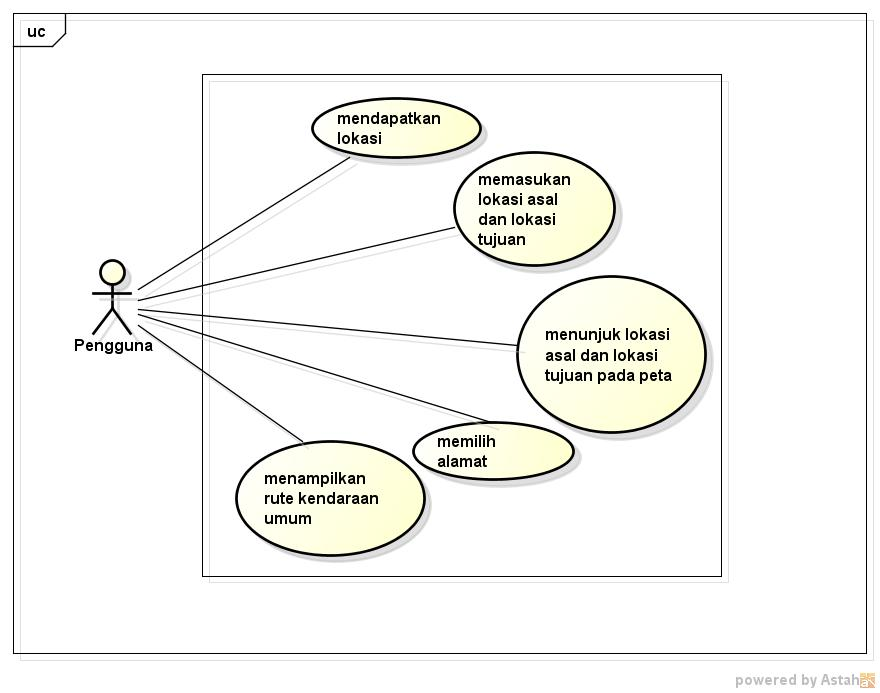
\includegraphics[scale=0.5]{Gambar/useCase_dan_Class/UseCase}
	\caption{Diagram \textit{Use Case}}
	\label{fig:UseCase}
\end{figure}

Skenario pencarian rute kendaraan umum dapat dilihat pada tabel~\ref{tab:mandapatLokasi} sampai tabel~\ref{tab:menampilkan}.
%\vtop{\hbox{\strut kalimat_1} \hbox{\strut kalimat_2}}
\begin{table}[H]
	\centering
		\begin{tabular}{ |p{2cm}|p{10cm}| }
			\hline
			Nama &  Mendapatkan lokasi perangkat\\ \hline
			Aktor & Pengguna  \\ \hline
			Deskripsi & Mendapatkan lokasi perangkat berada  \\ \hline
			Kondisi awal & \textit{textbox} masih kosong dan pengguna menekan tombol lokasi \\ \hline
			Kondisi akhir & Lokasi ditemukan dan \textit{textbox} berisi "here" \\ \hline
			Skenario utama & Pengguna menekan tombol lalu perangkat mencari lokasi perangkat dan \textit{textbox} berisi "here" \\ \hline
			Eksespsi & Lokasi tidak ditemukan jika GPS perangkat tidak aktif  \\ 
			\hline
		\end{tabular}
	\caption{Skenario Mendapatkan Lokasi untuk Masukan Lokasi Asal dan Lokasi Tujuan}
	\label{tab:mandapatLokasi}
\end{table}

\begin{table}[H]
	\centering
		\begin{tabular}{ |p{2cm}|p{10cm}| }
			\hline
			Nama &  Masukan pada \textit{textbox}\\ \hline
			Aktor & Pengguna  \\ \hline
			Deskripsi & Memasukan lokasi asal pengguna dan tujuan pengguna(masukan dapat berupa alamat, kordinat, atau tempat) \\ \hline
			Kondisi awal & \textit{textbox} masih dalam keadaan belum terisi \\ \hline
			Kondisi akhir & Lokasi awal dan tujuan sudah dimasukan   \\ \hline
			Skenario utama & Pengguna mengetikan lokasi awal dan tujuan pada \textit{textbox} yang sudah disediakan \\ \hline
			Eksespsi & Tidak ada  \\ 
			\hline
		\end{tabular}
	\caption{Skenario Memasukan Lokasi Asal dan Lokasi Tujuan pada \textit{textbox}}
	\label{tab:masukanLokasi}
\end{table}

\begin{table}[H]
	\centering
		\begin{tabular}{ |p{2cm}|p{10cm}| }
			\hline
			Nama &  Menunjuk lokasi pada peta\\ \hline
			Aktor & Pengguna  \\ \hline
			Deskripsi & Memasukan lokasi asal pengguna dan tujuan pengguna dengan menunjuk pada peta \\ \hline
			Kondisi awal & \textit{textbox} masih dalam keadaan belum terisi \\ \hline
			Kondisi akhir & \textit{textbox} terisi dengan "Maps"   \\ \hline
			Skenario utama & Pengguna menunjuk lokasi pada peta dan \textit{textbox} terisi dengan "Maps" \\ \hline
			Eksespsi & Tidak ada  \\ 
			\hline
		\end{tabular}
	\caption{Skenario Menunjuk Lokasi Asal dan Lokasi Tujuan pada Peta}
	\label{tab:lokasiPeta}
\end{table}

\begin{table}[H]
	\centering
		\begin{tabular}{ |p{2cm}|p{10cm}| }
			\hline
			Nama &  Memilih alamat\\ \hline
			Aktor & Pengguna  \\ \hline
			Deskripsi & Pengguna memilih alamat atau lokasi yang terkait masukan pengguna \\ \hline
			Kondisi awal & Lokasi awal dan lokasi tujuan terisi dan pengguna menekan tombol "Find" \\ \hline
			Kondisi akhir & Pengguna sudah memilih dan lokasi sudah dapat dipastikan  \\ \hline
			Skenario utama & Pengguna menekan tombol "Find". Sistem mengembalikan daftar yang berisi alamat atau tempat terkait masukan pengguna \\ \hline
			Eksespsi & Lokasi masukan pengguna tidak ditemukan  \\ 
			\hline
		\end{tabular}
	\caption{Skenario Memilih Alamat}
	\label{tab:memilihAlamat}
\end{table}

\begin{table}[H]
	\centering
		\begin{tabular}{ |p{2cm}|p{10cm}| }
			\hline
			Nama &  Menampilkan rute kendaraan umum\\ \hline
			Aktor & Pengguna  \\ \hline
			Deskripsi & Lokasi dari pengguna diolah menjadi rute kendaraan umum dari lokasi asal dan lokasi tujuan \\ \hline
			Kondisi awal & Lokasi sudah dapat dipastikan \\ \hline
			Kondisi akhir & Rute kendaraan umum dimunculkan pada peta dan dalam bentuk daftar \\ \hline
			Skenario utama & Lokasi dapat dipastikan sistem lalu istem akan memproses data masukan. Sistem akan mengembalikan hasil rute kendaraan umum pada peta dan dalam bentuk daftar \\ \hline
			Eksespsi & Rute kendaraan umum tidak ditemukan  \\ 
			\hline
		\end{tabular}
	\caption{Skenario Menampilkan Rute Kendaraan Umum}
	\label{tab:menampilkan}
\end{table}

%Analisis Kelas Diagram
\subsection{Kelas Diagram}
\label{lab:Kelas Diagram}
\hspace{0.5cm} Pembuatan kelas diagram didasarkan pada skenario pada sub-bab~\ref{lab:Diagram Use-Case dan Scenario}. Kelas diagram dapat dilihat pada gambar~\ref{fig:kelas}.

% Kelas
\begin{figure}[h]
	\centering
		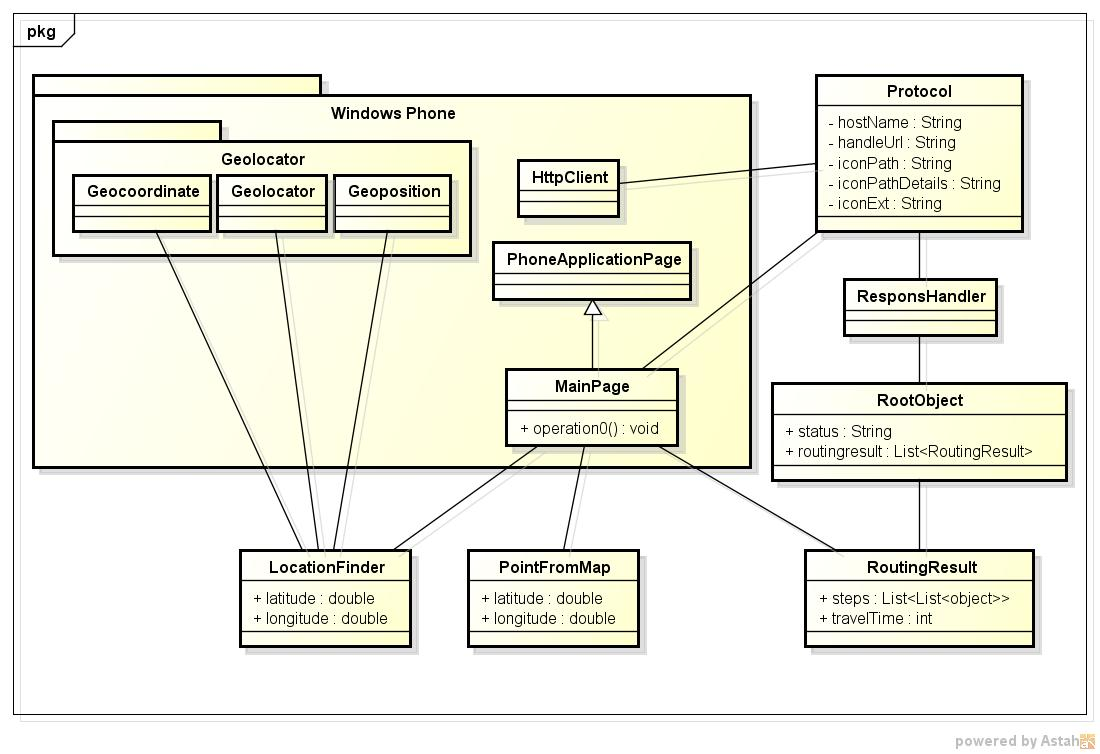
\includegraphics[scale=0.4]{Gambar/useCase_dan_Class/class}
	\caption{Diagram Kelas}
	\label{fig:kelas}
\end{figure}

Berikut deskripsi kelas pada gambar~\ref{fig:kelas}.
\begin{itemize}
	\item Kelas Protocol \\
	Merupakan kelas yang menampung semua alamat URL yang berhubungan dengan Kiri API. Semua pemanggilan ditangani oleh kelas ini.
	\item Kelas ResponsHandler \\
	Merupakan kelas yang menangani masukan dari pemanggilan layanan.
	\item Kelas RootObject \\
	Merupakan kelas untuk menampung status dan daftar dari layanan \textit{routing} Kiri API. Hasil kembalian dipisahkan di kelas ini untuk selanjutnya ditampung di kelas \textit{RoutingResult}. 
	\item Kelas RoutingResult \\
	Merupakan kelas untuk menampung setiap langkah dari rute sesuai masukan pengguna. Pada kelas ini juga rute digambarkan pada peta.
	\item Kelas PointFromMap \\
	Merupakan kelas yang dapat mengetahui lokasi yang ditunjuk pengguna pada peta. Kelas ini menyimpan lokasi yang ditunjuk pengguna dalam bentuk \textit{latitude} dan \textit{longitude}.
	\item Kelas LocationFinder \\
	Merupakan kelas yang digunakan untuk mencari lokasi. Kelas ini memanfaatkan kelas \textit{Geocoordinate} untuk mendapatkan lokasi. Setelah lokasi didapatkan dalam bentuk kelas \textit{Geoposition} maka diubah ke \textit{latitude} dan \textit{longitude}. 
\end{itemize}